\documentclass{report}

\usepackage[warn]{mathtext}
\usepackage[T2A]{fontenc}
\usepackage[utf8]{luainputenc}
\usepackage[english, russian]{babel}
\usepackage[pdftex]{hyperref}
\usepackage{tempora}
\usepackage[12pt]{extsizes}
\usepackage{listings}
\usepackage{color}
\usepackage{geometry}
\usepackage{enumitem}
\usepackage{multirow}
\usepackage{graphicx}
\usepackage{indentfirst}
\usepackage{amsmath}

\geometry{a4paper,top=2cm,bottom=2cm,left=2.5cm,right=1.5cm}
\setlength{\parskip}{0.5cm}
\setlist{nolistsep, itemsep=0.3cm,parsep=0pt}

\usepackage{listings}
\lstset{language=C++,
        basicstyle=\footnotesize,
		keywordstyle=\color{blue}\ttfamily,
		stringstyle=\color{red}\ttfamily,
		commentstyle=\color{green}\ttfamily,
		morecomment=[l][\color{red}]{\#}, 
		tabsize=4,
		breaklines=true,
  		breakatwhitespace=true,
  		title=\lstname,       
}

\makeatletter
\renewcommand\@biblabel[1]{#1.\hfil}
\makeatother

\begin{document}

\begin{titlepage}

\begin{center}
Министерство науки и высшего образования Российской Федерации
\end{center}

\begin{center}
Федеральное государственное автономное образовательное учреждение высшего образования \\
Национальный исследовательский Нижегородский государственный университет им. Н.И. Лобачевского
\end{center}

\begin{center}
Институт информационных технологий, математики и механики
\end{center}

\vspace{4em}

\begin{center}
\textbf{\LargeОтчет по лабораторной работе} \\
\end{center}
\begin{center}
\textbf{\Large Алгоритм Джарвиса поиска выпуклой оболочки} \\
\end{center}

\vspace{4em}

\newbox{\lbox}
\savebox{\lbox}{\hbox{text}}
\newlength{\maxl}
\setlength{\maxl}{\wd\lbox}
\hfill\parbox{7cm}{
\hspace*{5cm}\hspace*{-5cm}\textbf{Выполнил:} \\ студентка группы 381906-3 \\ Зайцева К.А. \\
\\
\hspace*{5cm}\hspace*{-5cm}\textbf{Проверил:}\\ доцент кафедры МОСТ, \\ кандидат технических наук \\ Сысоев А. В.\\
}
\vspace{\fill}

\begin{center} Нижний Новгород \\ 2022 \end{center}

\end{titlepage}

\setcounter{page}{2}

% Содержание
\tableofcontents
\newpage

% Введение
\section*{Введение}
\addcontentsline{toc}{section}{Введение}
\par Выпуклая оболочка множества точек — это выпуклое множество точек такое, что все остальные точки этого множества лежат внутри.
\par Для практических целей выпуклые оболочки полезны тем, что они компактно хранят всю необходимую информацию о множестве точек, что позволяет быстро отвечать на разнообразные запросы на этом множестве.
\par  В данной работе будет рассмотрен алгоритм Джарвиса поиска выпуклой оболочки. Который, также называют методом заворачивания подарка: мы как бы проходимся вокруг множества с оберткой, которая естественным образом заворачивается вокруг каждого следующего угла.
\newpage

% Постановка задачи
\section*{Постановка задачи}
\addcontentsline{toc}{section}{Постановка задачи}
\par Требуется разработать и реализовать последовательный и два параллельных алгоритма Джарвиса. Сравнить эффективность их работы. Подтвердить корректность. 
\par Параллельные алгоритмы разробатываются с помощью технологий openMP и TBB. 
\newpage

% Описание алгоритма
\section*{Описание алгоритма}
\addcontentsline{toc}{section}{Описание алгоритма}
Входным параметром является вектор с множеством точек. На выходе получаем вектор с выпуклой оболочкой для этого множества. \par 
Алгоритм описывается следующим образом: \par

\begin{enumerate}
\item Выбираем самую нижнюю точку p0 из множества. Добавим эту точку в оболочку.
\item Затем будем в цикле искать самую правую точку от последней добавленной (то есть точку с минимальным полярным углом относительно неё) и добавлять её в оболочку
\item Когда на каком-то шаге самой правой точкой станет p0, заканчиваем алгоритм. Оболочка замкнулась. 

\end{enumerate}
\newpage

% Описание схемы распараллеливания
\section*{Описание схемы распараллеливания}
\addcontentsline{toc}{section}{Описание схемы распараллеливания}
\par Параллельная версия для openMP и TBB заключается в следующем. Исходное множество точек разбивается на подмножества. Количество подмножеств равно количеству потоков. Для каждого из этих подмножеств параллельно запускается последовательный алгоритм Джарвиса. Из полученных выпуклых оболочек собирается новое множество точек. Для получения конечного результата для этого множества вновь используется последовательный алгоритм.

\newpage

% Описание программной реализации
\section*{Описание программной реализации}
\addcontentsline{toc}{section}{Описание программной реализации}
Программа состоит из заголовочного файла jarvis.h и двух файлов исходного кода  jarvis.cpp и main.cpp. В заголовочном файле находятся: структура Point, прототипы функций для последовательного и параллельных алгоритмов Джарвиса и прототип функции генерации множества точек. В jarvis.cpp - их реализация, а файл main.cpp содержит тесты, проверяющие корректность и эффективность работы программы.
\par Структура Point \par
\begin{lstlisting}
struct Point {
	Point() : x(0), y(0) {}
	Point(double x_, double y_) : x(x_), y(y_) {}
	double x;
	double y;
	bool operator<(const Point& other) const;
	bool operator==(const Point& other) const;
	bool operator!=(const Point& other) const;
	Point operator-(const Point& other) const;
};
\end{lstlisting}
\par Генерации множества точек \par
\begin{lstlisting}
std::vector<Point> Generate(int n);
\end{lstlisting}
\par  Вычисление определителя \par
\begin{lstlisting}
double cross(const Point& a, const Point& b);
\end{lstlisting}
\par Функция, проверяющая находиться ли точка c справа от отрезка [a, b]\par
\begin{lstlisting}
bool turn(const Point& a, const Point& b, const Point& c);
\end{lstlisting}
\par Последовательный алгоритм Джарвиса
\begin{lstlisting}
std::vector<Point> Jarvis(std::vector<Point> points);
\end{lstlisting}
\par Функция для параллельного алгоритма (OpenMP версия):
\begin{lstlisting}
std::vector<Point> Jarvis_parallel(std::vector<Point> points);
\end{lstlisting}
\par Функция для параллельного алгоритма (TBB версия):
\begin{lstlisting}
std::vector<Point> Jarvis_parallel_tbb(const std::vector<Point>& points);
\end{lstlisting}

\newpage

% Подтверждение корректности
\section*{Подтверждение корректности}
Для подтверждения корректности в программе представлен набор тестов, разработанных с  Google C++ Testing Framework. Кроме того, была реализована графическая интерпретация для этого алгоритма (рис.1). С ее помощью можно визуально оценить корректность программы. Параллельные алгоритмы сравниваются с последовательным, что также подтверждает корректность параллельных вариантов относительно последовательного. Также в тестах проверяется время работы и ускорение.


\begin{figure}[h]
	
	\centering
	
	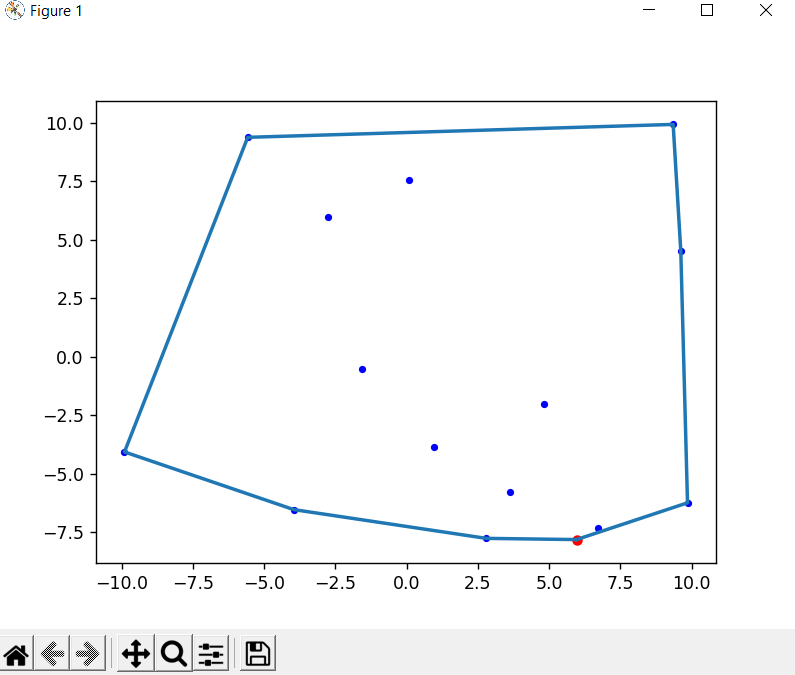
\includegraphics[width=0.8\linewidth]{graf.png}
	
	\caption{Пример графической интерпретации}
	
	\label{fig:mpr}
	
\end{figure}
\newpage

% Результаты экспериментов
\section*{Результаты экспериментов}
\addcontentsline{toc}{section}{Результаты экспериментов}
Вычислительные эксперименты для оценки эффективности работы параллельного алгоритма проводились на ПК со следующими характеристиками:
\begin{itemize}
\item Процессор: Intel(R) Core(TM) i7-8565U 1.80GHz, количество ядер: 4; логических процессов:8;
\item Оперативная память: 16 ГБ
\item Операционная система: Windows 10 Home.
\end{itemize}
\par Для экспериментов генерировалось множество из 1 000 000 точек.
\begin{table}[!h]
\caption{Результаты вычислительных экспериментов. Сравнение последовательного алгоритма с TBB}
\centering
\begin{tabular}{|p{4cm}|p{4cm}|p{4cm}|p{4cm}|}
\hline
Количество потоков & Последовательный алгоритм, сек & Параллельный алгоритм, сек & Ускорение  \\\hline
1 & 0.123812 &  0.136867 & 0.904612  \\\hline
2 & 0.0669834 & 0.0367999 & 1.82021  \\\hline
4 & 0.1015 & 0.0282299 & 3.5955  \\
\hline
\end{tabular}
\end{table}

\begin{table}[!h]
\caption{Результаты вычислительных экспериментов. Сравнение последовательного алгоритма с OpenMP}
\centering
\begin{tabular}{|p{4cm}|p{4cm}|p{4cm}|p{4cm}|}
\hline
Количество потоков & Последовательный алгоритм, сек & Параллельный алгоритм, сек & Ускорение  \\\hline
1 & 0.0819466 &  0.0823756 & 0.994792  \\\hline
2 & 0.0722183 & 0.0415884 & 1.7365  \\\hline
4 & 0.107535 & 0.0344418 & 3.12221  \\
\hline
\end{tabular}
\end{table}

\newpage

% Выводы из результатов экспериментов
\section*{Выводы из результатов экспериментов}
\addcontentsline{toc}{section}{Выводы из результатов экспериментов}
\par Из полученных данных видно, что параллельный алгоритм работает значительно быстрее, чем последовательный. Также видно, что ускорение увеличивается при увеличении количества потоков. Максимальное ускорение в 3,5 раза на 4 потоках. Сильных различий в производительности параллельных вариантов реализованных с помощью технологий TBB и openMP нет, так как использовалась одна и та же схема распараллеливания.

\newpage

\newpage

% Заключение
\section*{Заключение}
\addcontentsline{toc}{section}{Заключение}
В результате выполнения   данной лабораторной работы были разработаны последовательный и параллельные алгоритмы Джарвиса поиска выпуклой оболочки. Параллельное варианты реализованы при помощи технологий openMP и TBB. Проведенные тесты и графическая интерпретация показали корректность реализованных алгоритмов, а проведенные эксперименты показали, что параллельная версия алгоритма работает быстрее.

\newpage

% Литература
\section*{Литература}
\addcontentsline{toc}{section}{Литература}
\begin{enumerate}
\item Построение минимальных выпуклых оболочек [Электронный ресурс] // URL: \url{https://habr.com/ru/post/144921/}
\item Гергель В. П. Теория и практика параллельных вычислений. – 2007.
\item  Гергель В. П., Стронгин Р. Г. Основы параллельных вычислений для много-
процессорных вычислительных систем. – 2003.
\end{enumerate} 
\newpage

% Приложение
\section*{Приложение}
\addcontentsline{toc}{section}{Приложение}
\textbf{Последовательная версия}
\newline
\newline jarvis.h
\begin{lstlisting}
// Copyright 2022 Zaitseva Ksenia
#ifndef MODULES_TASK_1_ZAITSEVA_K_JARVIS_JARVIS_H_
#define MODULES_TASK_1_ZAITSEVA_K_JARVIS_JARVIS_H_

#include <fstream>
#include <iostream>
#include <limits>
#include <random>
#include <utility>
#include <vector>

struct Point {
	Point() : x(0), y(0) {}
	Point(double x_, double y_) : x(x_), y(y_) {}
	double x;
	double y;
	bool operator<(const Point& other) const;
	bool operator==(const Point& other) const;
	bool operator!=(const Point& other) const;
	Point operator-(const Point& other) const;
};

double cross(const Point& a, const Point& b);

bool turn(const Point& a, const Point& b, const Point& c);

std::vector<Point> Jarvis(std::vector<Point> points);

std::vector<Point> Generate(int n);

#endif  // MODULES_TASK_1_ZAITSEVA_K_JARVIS_JARVIS_H_
\end{lstlisting}
main.cpp
\begin{lstlisting}
// Copyright 2022 Zaitseva Ksenia
#include <gtest/gtest.h>
#include <vector>
#include "./jarvis.h"

TEST(Sequential, Test_Point_equal) {
	Point p1 = {0.2, 0.1};
	Point p2 = p1;
	ASSERT_TRUE(p2 == p1);
}

TEST(Sequential, Test_Point_less) {
	Point p1 = {0.2, 0.1};
	Point p2 = {-1.4, 0.0};
	ASSERT_TRUE(p2 < p1);
}

TEST(Sequential, Test_Point_minus) {
	Point p1 = {0.2, 0.1};
	Point p2 = {-1.4, 0.0};
	Point p3 = p1 - p2;
	EXPECT_EQ(Point(1.6, 0.1), p3);
}

TEST(Sequential, Test_Calc_Determinant) {
	Point p1 = {1.0, -2.0};
	Point p2 = {-1.0, 0.0};
	EXPECT_EQ(-2.0, cross(p1, p2));
}

TEST(Sequential, Test_and_Draw) {
	std::vector<Point> points = {{2.0, 1.0}, {-0.5, 1.0}, {-3.0, -1.5},
	{3.5, 1.0}, {0.5, 4.0},  {-4.5, -3.0},
	{-2.5, 3.5}};
	std::vector<Point> res = Jarvis(points);
	std::vector<Point> expected_res = {
	{-4.5, -3}, {3.5, 1}, {0.5, 4}, {-2.5, 3.5}};
	EXPECT_EQ(res, expected_res);
}

TEST(Sequential, Test_Generate_and_Draw) {
	std::vector<Point> points = Generate(10);
	std::ofstream fout("shell.txt");
	std::ofstream fout2("points.txt");
	std::vector<Point> res = Jarvis(points);
	for (std::size_t i = 0; i < res.size(); i++)
	fout << res[i].x << std::endl << res[i].y << std::endl;
	fout << res[0].x << std::endl << res[0].y << std::endl;
	for (auto i = points.begin(); i != points.end(); i++)
	fout2 << i->x << std::endl << i->y << std::endl;
	fout.close();
	fout2.close();
}
\end{lstlisting}
jarvis.cpp
\begin{lstlisting}
// Copyright 2022 Zaitseva Ksenia
#include "../../modules/task_1/zaitseva_k_jarvis/jarvis.h"

bool Point::operator<(const Point& other) const {
	if ((y < other.y) || ((y == other.y) && (x > other.x)))
		return 1;
	else
		return 0;
}

bool Point::operator==(const Point& other) const {
	return (std::fabs(x - other.x) <
	1000 * std::numeric_limits<double>::epsilon()) &&
	(std::fabs(y - other.y) <
	1000 * std::numeric_limits<double>::epsilon());
}

bool Point::operator!=(const Point& other) const { return !(*this == other); }

Point Point::operator-(const Point& other) const {
	return Point(x - other.x, y - other.y);
}

double cross(const Point& a, const Point& b) { return a.x * b.y - b.x * a.y; }

bool turn(const Point& a, const Point& b, const Point& c) {
	double det = cross(b - a, c - a);
	if (det > 0.0) {
		return 0;
	} else if (det < 0.0) {
		return 1;
	} else if (det == 0.0) {
		double distans_a_b =
		std::sqrt((b.x - a.x) * (b.x - a.x) * (b.y - a.y) * (b.y - a.y));
		double distans_a_c =
		std::sqrt((c.x - a.x) * (c.x - a.x) * (c.y - a.y) * (c.y - a.y));
		if (distans_a_c > distans_a_b)
			return 1;
		else
			return 0;
	}
	return 0;
}

std::vector<Point> Jarvis(std::vector<Point> points) {
	Point p0 = points[0];
	int k = 0;
	for (std::size_t i = 1; i < points.size(); i++) {
		if (points[i] < p0) {
			p0 = points[i];
			k = i;
		}
	}
	std::swap(points[k], points[0]);
	Point p_next, p_i = p0;
	std::size_t i = 1;
	for (i = 1; i < points.size(); i++) {
		p_next = points[i];
		k = i;
		for (std::size_t j = i + 1; j < points.size(); j++) {
			if (turn(p_i, p_next, points[j])) {
				p_next = points[j];
				k = j;
			}
		}
		if (turn(p_i, p_next, p0)) {
			break;
		}
		std::swap(points[k], points[i]);
		p_i = p_next;
	}
	return std::vector<Point>(points.begin(), points.begin() + i);
}

std::vector<Point> Generate(int n) {
	std::vector<Point> res;
	std::default_random_engine engine;
	std::uniform_real_distribution<double> uniform(-10, 10);
	for (int i = 0; i < n; i++) {
		res.push_back(Point(uniform(engine), uniform(engine)));
	}
	return res;
}

\end{lstlisting}

\textbf{TBB версия}
\newline
\newline jarvis.h
\begin{lstlisting}
// Copyright 2022 Zaitseva Ksenia
#ifndef MODULES_TASK_3_ZAITSEVA_K_JARVIS_JARVIS_H_
#define MODULES_TASK_3_ZAITSEVA_K_JARVIS_JARVIS_H_

#include <fstream>
#include <iostream>
#include <limits>
#include <random>
#include <utility>
#include <vector>

#include "tbb/tbb.h"

struct Point {
	Point() : x(0), y(0) {}
	Point(double x_, double y_) : x(x_), y(y_) {}
	double x;
	double y;
	bool operator<(const Point& other) const;
	bool operator==(const Point& other) const;
	bool operator!=(const Point& other) const;
	Point operator-(const Point& other) const;
};

double cross(const Point& a, const Point& b);

bool turn(const Point& a, const Point& b, const Point& c);

std::vector<Point> Jarvis(std::vector<Point> points);

std::vector<Point> Generate(int n);

std::vector<Point> Jarvis_parallel_tbb(const std::vector<Point>& points);

#endif  // MODULES_TASK_3_ZAITSEVA_K_JARVIS_JARVIS_H_

\end{lstlisting}
jarvis.cpp
\begin{lstlisting}
// Copyright 2022 Zaitseva Ksenia
#include "../../modules/task_3/zaitseva_k_jarvis/jarvis.h"

bool Point::operator<(const Point& other) const {
if ((y < other.y) || ((y == other.y) && (x > other.x)))
	return 1;
else
	return 0;
}

bool Point::operator==(const Point& other) const {
	return (std::fabs(x - other.x) <
	1000 * std::numeric_limits<double>::epsilon()) &&
	(std::fabs(y - other.y) <
	1000 * std::numeric_limits<double>::epsilon());
}

bool Point::operator!=(const Point& other) const { return !(*this == other); }

Point Point::operator-(const Point& other) const {
	return Point(x - other.x, y - other.y);
}

double cross(const Point& a, const Point& b) { return a.x * b.y - b.x * a.y; }

bool turn(const Point& a, const Point& b, const Point& c) {
	double det = cross(b - a, c - a);
	if (det > 0.0) {
		return 0;
	} else if (det < 0.0) {
		return 1;
	} else if (det == 0.0) {
	double distans_a_b =
		std::sqrt((b.x - a.x) * (b.x - a.x) * (b.y - a.y) * (b.y - a.y));
	double distans_a_c =
		std::sqrt((c.x - a.x) * (c.x - a.x) * (c.y - a.y) * (c.y - a.y));
	if (distans_a_c > distans_a_b)
		return 1;
	else
		return 0;
	}
	return 0;
}

std::vector<Point> Jarvis(std::vector<Point> points) {
	Point p0 = points[0];
	int k = 0;
	for (std::size_t i = 1; i < points.size(); i++) {
		if (points[i] < p0) {
			p0 = points[i];
			k = i;
		}
	}
	std::swap(points[k], points[0]);
	Point p_next, p_i = p0;
	std::size_t i = 1;
	for (i = 1; i < points.size(); i++) {
		p_next = points[i];
		k = i;
		for (std::size_t j = i + 1; j < points.size(); j++) {
			if (turn(p_i, p_next, points[j])) {
				p_next = points[j];
				k = j;
			}
		}
		if (turn(p_i, p_next, p0)) {
			break;
		}
		std::swap(points[k], points[i]);
		p_i = p_next;
	}
	return std::vector<Point>(points.begin(), points.begin() + i);
}

std::vector<Point> Generate(int n) {
	std::vector<Point> res;
	std::default_random_engine engine;
	std::uniform_real_distribution<double> uniform(-10, 10);
	for (int i = 0; i < n; i++) {
		res.push_back(Point(uniform(engine), uniform(engine)));
	}
	return res;
}

std::vector<Point> Jarvis_parallel_tbb(const std::vector<Point>& points) {
	int num_threads = 4;
	std::vector<std::vector<Point>> shells(num_threads);
	int step = points.size() / num_threads;
	tbb::task_scheduler_init init(num_threads);
	tbb::parallel_for(tbb::blocked_range<int>(0, num_threads),
	[=, &shells, &points](const tbb::blocked_range<int>& r) {
		int th_num = r.begin();
		auto end = th_num == (num_threads - 1)
		? points.end()
		: points.begin() + (th_num + 1) * step;
		shells[th_num] = Jarvis(std::vector<Point>(
		points.begin() + th_num * step, end));
	});
	std::vector<Point> new_points;
	for (int i = 0; i < num_threads; i++)
	std::copy(shells[i].begin(), shells[i].end(),
	std::back_inserter(new_points));
	return Jarvis(new_points);
}

\end{lstlisting}
main.cpp
\begin{lstlisting}
// Copyright 2022 Zaitseva Ksenia
#include <gtest/gtest.h>

#include <chrono> // NOLINT [build/c++11]
#include <vector>
#include <omp.h>

#include "./jarvis.h"

TEST(TBB, Test_Point_equal) {
	Point p1 = {0.2, 0.1};
	Point p2 = p1;
	ASSERT_TRUE(p2 == p1);
}

TEST(TBB, Test_Point_less) {
	Point p1 = {0.2, 0.1};
	Point p2 = {-1.4, 0.0};
	ASSERT_TRUE(p2 < p1);
}

TEST(TBB, Test_Point_minus) {
	Point p1 = {0.2, 0.1};
	Point p2 = {-1.4, 0.0};
	Point p3 = p1 - p2;
	EXPECT_EQ(Point(1.6, 0.1), p3);
}

TEST(TBB, Test_Calc_Determinant) {
	Point p1 = {1.0, -2.0};
	Point p2 = {-1.0, 0.0};
	EXPECT_EQ(-2.0, cross(p1, p2));
}

TEST(TBB, Test_Jarvis) {
	std::vector<Point> points = {{2.0, 1.0}, {-0.5, 1.0}, {-3.0, -1.5},
	{3.5, 1.0}, {0.5, 4.0},  {-4.5, -3.0},
	{-2.5, 3.5}};
	std::vector<Point> res = Jarvis_parallel_tbb(points);
	std::vector<Point> expected_res = {
	{-4.5, -3}, {3.5, 1}, {0.5, 4}, {-2.5, 3.5}};
	EXPECT_EQ(res, expected_res);
}

TEST(TBB, Test_Generate_and_Draw) {
	std::vector<Point> points = Generate(10);
	std::ofstream fout("shell.txt");
	std::ofstream fout2("points.txt");
	std::vector<Point> res = Jarvis_parallel_tbb(points);
	for (std::size_t i = 0; i < res.size(); i++)
	fout << res[i].x << std::endl << res[i].y << std::endl;
	fout << res[0].x << std::endl << res[0].y << std::endl;
	for (auto i = points.begin(); i != points.end(); i++)
	fout2 << i->x << std::endl << i->y << std::endl;
	fout.close();
	fout2.close();
}

TEST(TBB, Test_Compare_with_Seq) {
	double t1, t2, time_par, time_seq;
	std::vector<Point> points = Generate(1000000);
	t1 = omp_get_wtime();
	std::vector<Point> res_par = Jarvis_parallel_tbb(points);
	t2 = omp_get_wtime();
	time_par = t2 - t1;
	t1 = omp_get_wtime();
	std::vector<Point> res_seq = Jarvis(points);
	t2 = omp_get_wtime();
	time_seq = t2 - t1;
	std::cout << "Sequential = " << time_seq << std::endl;
	std::cout << "Parallel = " << time_par << std::endl;
	std::cout << "Parallel version faster on " << time_seq / time_par
	<< std::endl;
	EXPECT_EQ(res_par, res_seq);
}

\end{lstlisting}

\textbf{openMP версия}
\newline
\newline jarvis.h
\begin{lstlisting}
// Copyright 2022 Zaitseva Ksenia
#ifndef MODULES_TASK_2_ZAITSEVA_K_JARVIS_JARVIS_H_
#define MODULES_TASK_2_ZAITSEVA_K_JARVIS_JARVIS_H_

#include <omp.h>

#include <fstream>
#include <iostream>
#include <limits>
#include <random>
#include <utility>
#include <vector>

struct Point {
	Point() : x(0), y(0) {}
	Point(double x_, double y_) : x(x_), y(y_) {}
	double x;
	double y;
	bool operator<(const Point& other) const;
	bool operator==(const Point& other) const;
	bool operator!=(const Point& other) const;
	Point operator-(const Point& other) const;
};

double cross(const Point& a, const Point& b);

bool turn(const Point& a, const Point& b, const Point& c);

std::vector<Point> Jarvis(std::vector<Point> points);

std::vector<Point> Generate(int n);

std::vector<Point> Jarvis_parallel(std::vector<Point> points);

#endif  // MODULES_TASK_2_ZAITSEVA_K_JARVIS_JARVIS_H_

\end{lstlisting}
jarvis.cpp
\begin{lstlisting}
// Copyright 2022 Zaitseva Ksenia
#include "../../modules/task_2/zaitseva_k_jarvis/jarvis.h"

bool Point::operator<(const Point& other) const {
	if ((y < other.y) || ((y == other.y) && (x > other.x)))
		return 1;
	else
		return 0;
}

bool Point::operator==(const Point& other) const {
	return (std::fabs(x - other.x) <
	1000 * std::numeric_limits<double>::epsilon()) &&
	(std::fabs(y - other.y) <
	1000 * std::numeric_limits<double>::epsilon());
}

bool Point::operator!=(const Point& other) const { return !(*this == other); }

Point Point::operator-(const Point& other) const {
	return Point(x - other.x, y - other.y);
}

double cross(const Point& a, const Point& b) { return a.x * b.y - b.x * a.y; }

bool turn(const Point& a, const Point& b, const Point& c) {
	double det = cross(b - a, c - a);
	if (det > 0.0) {
		return 0;
	} else if (det < 0.0) {
		return 1;
	} else if (det == 0.0) {
		double distans_a_b =
		std::sqrt((b.x - a.x) * (b.x - a.x) * (b.y - a.y) * (b.y - a.y));
		double distans_a_c =
		std::sqrt((c.x - a.x) * (c.x - a.x) * (c.y - a.y) * (c.y - a.y));
		if (distans_a_c > distans_a_b)
			return 1;
		else
			return 0;
	}
	return 0;
}

std::vector<Point> Jarvis(std::vector<Point> points) {
	Point p0 = points[0];
	int k = 0;
	for (std::size_t i = 1; i < points.size(); i++) {
		if (points[i] < p0) {
			p0 = points[i];
			k = i;
		}
	}
	std::swap(points[k], points[0]);
	Point p_next, p_i = p0;
	std::size_t i = 1;
	for (i = 1; i < points.size(); i++) {
		p_next = points[i];
		k = i;
		for (std::size_t j = i + 1; j < points.size(); j++) {
			if (turn(p_i, p_next, points[j])) {
				p_next = points[j];
				k = j;
			}
		}
		if (turn(p_i, p_next, p0)) {
			break;
		}
		std::swap(points[k], points[i]);
		p_i = p_next;
	}
	return std::vector<Point>(points.begin(), points.begin() + i);
}

std::vector<Point> Generate(int n) {
	std::vector<Point> res;
	std::default_random_engine engine;
	std::uniform_real_distribution<double> uniform(-10, 10);
	for (int i = 0; i < n; i++) {
		res.push_back(Point(uniform(engine), uniform(engine)));
	}
	return res;
}

std::vector<Point> Jarvis_parallel(std::vector<Point> points) {
	int num_threads = 4;
	std::vector<std::vector<Point>> shells(num_threads);
	omp_set_num_threads(num_threads);
	int step = points.size() / num_threads;
#pragma omp parallel
{
	int th_num = omp_get_thread_num();
	auto end = th_num == (num_threads - 1) ? points.end()
	: points.begin() + (th_num + 1) * step;
	shells[th_num] =
		Jarvis(std::vector<Point>(points.begin() + th_num * step, end));
}
	std::vector<Point> new_points;
	for (int i = 0; i < num_threads; i++)
		std::copy(shells[i].begin(), shells[i].end(), std::back_inserter(new_points));
	return Jarvis(new_points);
}


\end{lstlisting}
main.cpp
\begin{lstlisting}
// Copyright 2022 Zaitseva Ksenia
#include <gtest/gtest.h>

#include <vector>

#include "./jarvis.h"

TEST(OpenMP, Test_Point_equal) {
	Point p1 = {0.2, 0.1};
	Point p2 = p1;
	ASSERT_TRUE(p2 == p1);
}

TEST(OpenMP, Test_Point_less) {
	Point p1 = {0.2, 0.1};
	Point p2 = {-1.4, 0.0};
	ASSERT_TRUE(p2 < p1);
}

TEST(OpenMP, Test_Point_minus) {
	Point p1 = {0.2, 0.1};
	Point p2 = {-1.4, 0.0};
	Point p3 = p1 - p2;
	EXPECT_EQ(Point(1.6, 0.1), p3);
}

TEST(OpenMP, Test_Calc_Determinant) {
	Point p1 = {1.0, -2.0};
	Point p2 = {-1.0, 0.0};
	EXPECT_EQ(-2.0, cross(p1, p2));
}

TEST(OpenMP, Test_Jarvis) {
	std::vector<Point> points = {{2.0, 1.0}, {-0.5, 1.0}, {-3.0, -1.5},
	{3.5, 1.0}, {0.5, 4.0},  {-4.5, -3.0},
	{-2.5, 3.5}};
	std::vector<Point> res = Jarvis_parallel(points);
	std::vector<Point> expected_res = {
	{-4.5, -3}, {3.5, 1}, {0.5, 4}, {-2.5, 3.5}};
	EXPECT_EQ(res, expected_res);
}

TEST(OpenMP, Test_Generate_and_Draw) {
	std::vector<Point> points = Generate(1000);
	std::ofstream fout("shell.txt");
	std::ofstream fout2("points.txt");
	std::vector<Point> res = Jarvis_parallel(points);
	for (std::size_t i = 0; i < res.size(); i++)
	fout << res[i].x << std::endl << res[i].y << std::endl;
	fout << res[0].x << std::endl << res[0].y << std::endl;
	for (auto i = points.begin(); i != points.end(); i++)
	fout2 << i->x << std::endl << i->y << std::endl;
	fout.close();
	fout2.close();
}

TEST(OpenMP, Test_Compare_with_Seq) {
	double t1, t2, time_par, time_seq;
	std::vector<Point> points = Generate(1000000);
	t1 = omp_get_wtime();
	std::vector<Point> res_par = Jarvis_parallel(points);
	t2 = omp_get_wtime();
	time_par = t2 - t1;
	t1 = omp_get_wtime();
	std::vector<Point> res_seq = Jarvis(points);
	t2 = omp_get_wtime();
	time_seq = t2 - t1;
	std::cout << "Sequential = " << time_seq << std::endl;
	std::cout << "Parallel = " << time_par << std::endl;
	std::cout << "Parallel version faster on " << time_seq / time_par
	<< std::endl;
	EXPECT_EQ(res_par, res_seq);
}

\end{lstlisting}

\end{document}